\chapter{Arhitektura i dizajn sustava}
		
		\noindent\text Arhitektura sustava koji projektiramo može se razdvojiti na dvije cjeline: web aplikaciju
		i bazu podataka.\par
		\textit{}\\
		\text Web aplikacija sastoji se od web preglednika i web poslužitelja.\par
		
		 \underbar{Web preglednik} jest grafički prikaz implementacije naše aplikacije koji je lako razumljiv korisniku i njim se korisnik služi kako bi pregledao web-stranicu ili multimedijalni sadržaj pohranjen na njoj. Uloga preglednika prevođenje je koda u lako razumljiv grafički prikaz i omogućavanje korisniku slanje upita i zahtjeva web poslužitelju.\par
		
		\underline{Web poslužitelj} služi za komunikaciju i obradu zahtjeva između korisnika i aplikacije. Koristi protokol HTTP za komunikaciju i prosljeđuje HTTP zahtjev aplikaciji. Aplikacija možebitno pristupa bazi podataka i potom vrati preko poslužitelja HTML dokument kao odgovor.\par
		\textit{}\\
		\text Programska podrška izvedena je kao Node.js aplikacija pisana u jeziku JavaScript. Pohrana podataka izvedena preko PostgreSQL baze podataka. \\
		
		\noindent\text Izabrana arhitektura sustava temeljena je na \textbf{MVC modelu}. MVC model omogućava odvojeni razvoj pojedinih dijelova web aplikacije (što dovodi do jednostavnijeg razvoja), ispitivanje i nadogradnju sustava. MVC model varijacija je arhitekture zasnovane na događajima (event based architecture): komponente se ne pozivaju eksplicitno, već reagiraju na događaje, odn. signale koje generiraju druge komponente. Smanjena je međuovisnost između korisničkog sučelja i ostatka sustava.
		
MVC model sastoji se od sljedećih dijelova:\par
	\begin{itemize}
		\item 	\textbf{Model (Model)} jest dinamička struktura podataka, neovisna o korisničkom sučelju; zadužen za upravljanje logikom i tokom podataka aplikacije.
		\item 	\textbf{Pogled (View)} predstavlja grafički prikaz podataka i funkcionalnosti
		\item 	\textbf{Naglednikom (Controller)} korisnik se služi za slanje zahtjeva i ovisno o sadržaju tih zahtjeva naglednik ih proslijedi modelu ili pogledu.		
	\end{itemize}

	
		

		

				
		\section{Baza podataka}
			
			
		
		
		    \noindent Za potrebe našeg sustava koristit ćemo relacijsku bazu podataka koja
            svojom strukturom olakšava modeliranje stvarnog svijeta. Gradivna jedinka
            baze je relacija, odnosno tablica koja je definirana svojim imenom i 
            skupom atributa. Zadaća baze podataka brza je i jednostavna pohrana, 
            izmjena i dohvat podataka za daljnju obradu.
            Baza podataka ove aplikacije sastoji se od sljedećih entiteta:
            
            \begin{packed_item}
                \item Korisnik
                \item Poslovnica
                \item Recenzija
                \item Rezervacija
                \item Session
                \item Vozilo
            \end{packed_item}
		
			\subsection{Opis tablica}
			

				%\textit{Svaku tablicu je potrebno opisati po zadanom predlošku. Lijevo se nalazi točno ime varijable u bazi podataka, u sredini se nalazi tip podataka, a desno se nalazi opis varijable. Svjetlozelenom bojom označite primarni ključ. Svjetlo plavom označite strani ključ} \newline
				
				
				\noindent \textbf{Korisnik} \quad Ovaj entitet sadržava sve važne informacije o korisniku aplikacije. Sadrži atribute: korisnickoIme, ime, prezime, email, lozinka, brojMobitela i uloga. Ovaj entitet u vezi je
                \textit{One-to-Many} s entitetom Rezervacija preko atributa korisnickoIme korisnika i u vezi \textit{One-to-Many} s entitetom Session preko korisničkog imena. Atribut sess iz tablice Session jest kolačić tipa json koji u sebi sadrži sve podatke o korisniku. 
                
                \begin{longtabu} to \textwidth {|X[6, l]|X[6, l]|X[20, l]|}
					
					\hline \multicolumn{3}{|c|}{\textbf{Korisnik}}	 \\[3pt] \hline
					\endfirsthead
					
					\hline \multicolumn{3}{|c|}{\textbf{Korisnik}}	 \\[3pt] \hline
					\endhead
					
					\hline 
					\endlastfoot
					
					\textcolor{LightGreen}{korisnickoIme}  & VARCHAR	&  	korisničko ime korisnika koje je ujedno i jedinstveni identifikator\\ \hline
					ime	& VARCHAR &   ime korisnika\\ \hline
					prezime	& VARCHAR &   prezime korisnika\\ \hline
					email & VARCHAR &   e-mail adresa korisnika\\ \hline
					lozinka	& VARCHAR &   lozinka korisnika\\ \hline
					brojMobitela	& VARCHAR &   broj mobitela korisnika\\ \hline 
					uloga	& VARCHAR &   definira razinu ovlasti korisnika\\ \hline
					
					
				\end{longtabu}
				
				\newpage
				\noindent \textbf{Poslovnica} \quad Ovaj entitet sadržava sve važne informacije o poslovnici. Sadrži atribute: idPoslovnica i lokacija.
				
				\begin{longtabu} to \textwidth {|X[6, l]|X[6, l]|X[20, l]|}
					
					\hline \multicolumn{3}{|c|}{\textbf{Poslovnica}}	 \\[3pt] \hline
					\endfirsthead
					
					\hline \multicolumn{3}{|c|}{\textbf{Poslovnica}}	 \\[3pt] \hline
					\endhead
					
					\hline 
					\endlastfoot
					
					\textcolor{LightGreen}{idPoslovnica} & INT	&  	jedinstveni identifikator poslovnice\\ \hline
					lokacija	& VARCHAR &   adresa poslovnice\\ \hline
					
					
				\end{longtabu}
				
				\noindent \textbf{Recenzija} \quad Ovaj entitet sadržava sve važne informacije vezane za osvrt korisnika o pruženoj usluzi. Sadrži atribute: idRecenzija,
                ocjena, opis i korisnickoIme.
                Ovaj entitet u vezi je \textit{One-to-One} s entitetom Rezervacija preko atributa idRezervacija.
                
                \begin{longtabu} to \textwidth {|X[6, l]|X[6, l]|X[20, l]|}
					
					\hline \multicolumn{3}{|c|}{\textbf{Recenzija}}	 \\[3pt] \hline
					\endfirsthead
					
					\hline \multicolumn{3}{|c|}{\textbf{Recenzija}}	 \\[3pt] \hline
					\endhead
					
					\hline 
					\endlastfoot
					
					\textcolor{LightGreen}{idRecenzija} & INT	&  	jedinstveni identifikator recenzije\\ \hline
					ocjena	& INT &   ocjena za uslugu\\ \hline
					opis	& VARCHAR &   komentar na ocjenu usluge\\ \hline
					\textcolor{LightBlue}{korisnickoIme}	& VARCHAR &   jedinstveni identifikator korisnika, (korisnik.korisničko ime)	\\ \hline 
					
				\end{longtabu}
				
				\noindent \textbf{Rezervacija} \quad Ovaj entitet sadržava sve važne informacije vezane uz najam vozila. Sadrži atribute: idRezervacija, vrijemeRezervacije, vrijemePreuzimanja, vrijemeZavršetka, lokacijaPreuzimanja, lokacijaOstavljanja, korisnickoIme, registracija i status. Ovaj entitet u vezi je \textit{Many-to-One} s entitetom Korisnik preko korisničkog imena, u vezi \textit{One-to-One} s entitetom Recenzija preko atributa idRezervacija i u vezi \textit{Many-to-One} s entitetom Vozilo preko registracije. Ima dvije veze \textit{Many-to-One} s entitetom Poslovnica koje ostvaruje preko dva atributa (lokacijaPreuzimanja i lokacijaOstavljanja) koji se spajaju na atribut lokacija entiteta Poslovnica. 
                
                \begin{longtabu} to \textwidth {|X[6, l]|X[6, l]|X[20, l]|}
					
					\hline \multicolumn{3}{|c|}{\textbf{Rezervacija}}	 \\[3pt] \hline
					\endfirsthead
					
					\hline \multicolumn{3}{|c|}{\textbf{Rezervacija}}	 \\[3pt] \hline
					\endhead
					
					\hline 
					\endlastfoot
					
					\textcolor{LightGreen}{idRezervacija} & INT	&  	jedinstveni identifikator rezervacije\\ \hline
					vrijeme- Rezervacije & TIMESTAMP &   trenutak u kojem je napravljena rezervacija\\ \hline
					vrijeme- Preuzimanja	& TIMESTAMP &   trenutak u kojem je korisnik preuzeo iznajmljeno vozilo \\ \hline
					vrijeme- Završetka & TIMESTAMP &   trenutak u kojem je korisnik vratio iznajmljeno vozilo\\ \hline
					lokacija- Preuzimanja	& VARCHAR &   lokacija na kojoj se preuzima iznajmljeno vozilo\\ \hline
					lokacija- Ostavljanja	& VARCHAR &   lokacija na koju se vraća iznajmljeno vozilo\\ \hline 
					\textcolor{LightBlue}{korisnickoIme}	& VARCHAR &   jedinstveni identifikator korisnika (korisnik.korisnickoIme)\\ \hline
					\textcolor{LightBlue}{registracija}	& VARCHAR &   jedinstveni identifikator vozila (vozilo.registracija)\\ \hline
					status	& VARCHAR &   definira je li rezervacija aktivna ili završena\\ \hline
					
					
				\end{longtabu}
				
				\noindent \textbf{Session} \quad Ovaj entitet sadržava sve važne informacije o sjednici web stranice. Sjednica predstavlja slijed vremenski omeđenih i logički povezanih transakcija između pojedinog klijenta i poslužitelja. Sadrži atribute: sid, sess i expire. Sid, tj. jedinstveni identifikator sjednice pridijeljen je svakoj transakciji koja pripada određenoj sjednici. Atribut sess tipa json jest kolačić koji u sebi sadrže sve podatke o korisniku koji je započeo sjednicu. Ovaj entitet u vezi je \textit{One-to-One} s korisnikom.

                
                \begin{longtabu} to \textwidth {|X[6, l]|X[6, l]|X[20, l]|}
					
					\hline \multicolumn{3}{|c|}{\textbf{Session}}	 \\[3pt] \hline
					\endfirsthead
					
					\hline \multicolumn{3}{|c|}{\textbf{Session}}	 \\[3pt] \hline
					\endhead
					
					\hline 
					\endlastfoot
					
					\textcolor{LightGreen}{sId} & INT	&  	jedinstveni identifikator sjednice\\ \hline
					sess	& JSON &   kolačić sjednice\\ \hline
					expire	& TIMESTAMP &  vrijeme isteka sjednice \\ \hline

					
				\end{longtabu}
				
				\noindent \textbf{Vozilo} \quad Ovaj entitet sadržava sve važne informacije o vozilu koje se iznajmljuje. Sadrži atribute: registracija, marka, model, kategorija, cijenaDan i slikaURL. Ovaj entitet u vezi je \textit One-To-Many s entitetom Rezervacija preko registracije. 
                
                \begin{longtabu} to \textwidth {|X[6, l]|X[6, l]|X[20, l]|}
					
					\hline \multicolumn{3}{|c|}{\textbf{Vozilo}}	 \\[3pt] \hline
					\endfirsthead
					
					\hline \multicolumn{3}{|c|}{\textbf{Vozilo}}	 \\[3pt] \hline
					\endhead
					
					\hline 
					\endlastfoot
					
					\textcolor{LightGreen}{registracija} & VARCHAR	&  	jedinstveni identifikator vozila\\ \hline
					marka	& VARCHAR &   oznaka porijekla vozila\\ \hline
					model	& VARCHAR &   model vozila \\ \hline
					kategorija & VARCHAR &   kategorija vozila: niža, srednja ili viša\\ \hline
					cijenaDan	& NUMERIC &   cijena dnevnog najma \\ \hline
					slikaURL	& VARCHAR &   URL fotografije vozila\\ \hline 
					
					
				\end{longtabu}
			
			
			\newpage\subsection{Dijagram baze podataka}
			
			 \begin{figure}[hp]
                    \centering
                    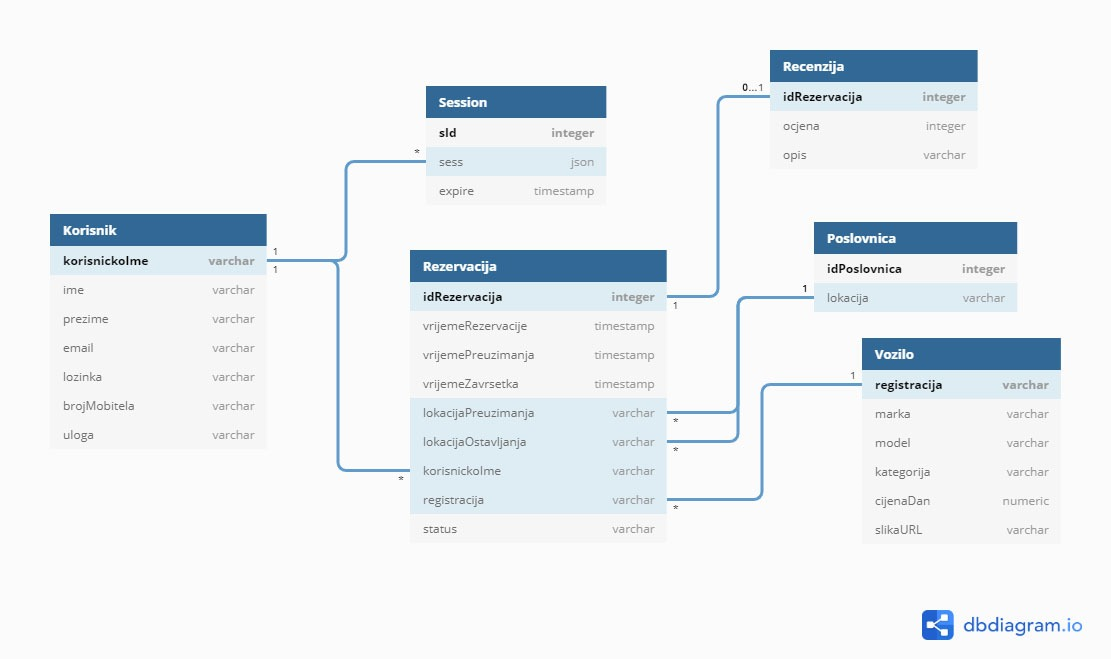
\includegraphics[width=15cm]{slike/ER_dijagram.png}
                    \caption{ER dijagram baze podataka}
                    \label{fig:useCase-2}
                \end{figure}
			
			
		\newpage
		\section{Dijagram razreda}
			
			Na slikama \ref{fig:classDiagram-1}, \ref{fig:classDiagram-2} i \ref{fig:classDiagram-3} prikazani su razredi \textit{backend} dijela MVC modela aplikacije. Razredi prikazani na slici \ref{fig:classDiagram-1} nasljeđuju Controller razred. Metode implementirane u tim razredima informacijom manipuliraju objektima i to tzv. \textit{Data Transfer Object}, ili, kako smo ih u daljnjem tekstu nazivali, DTO-ima.\\
	
	        
	        \begin{figure}[hp]
                \centering
                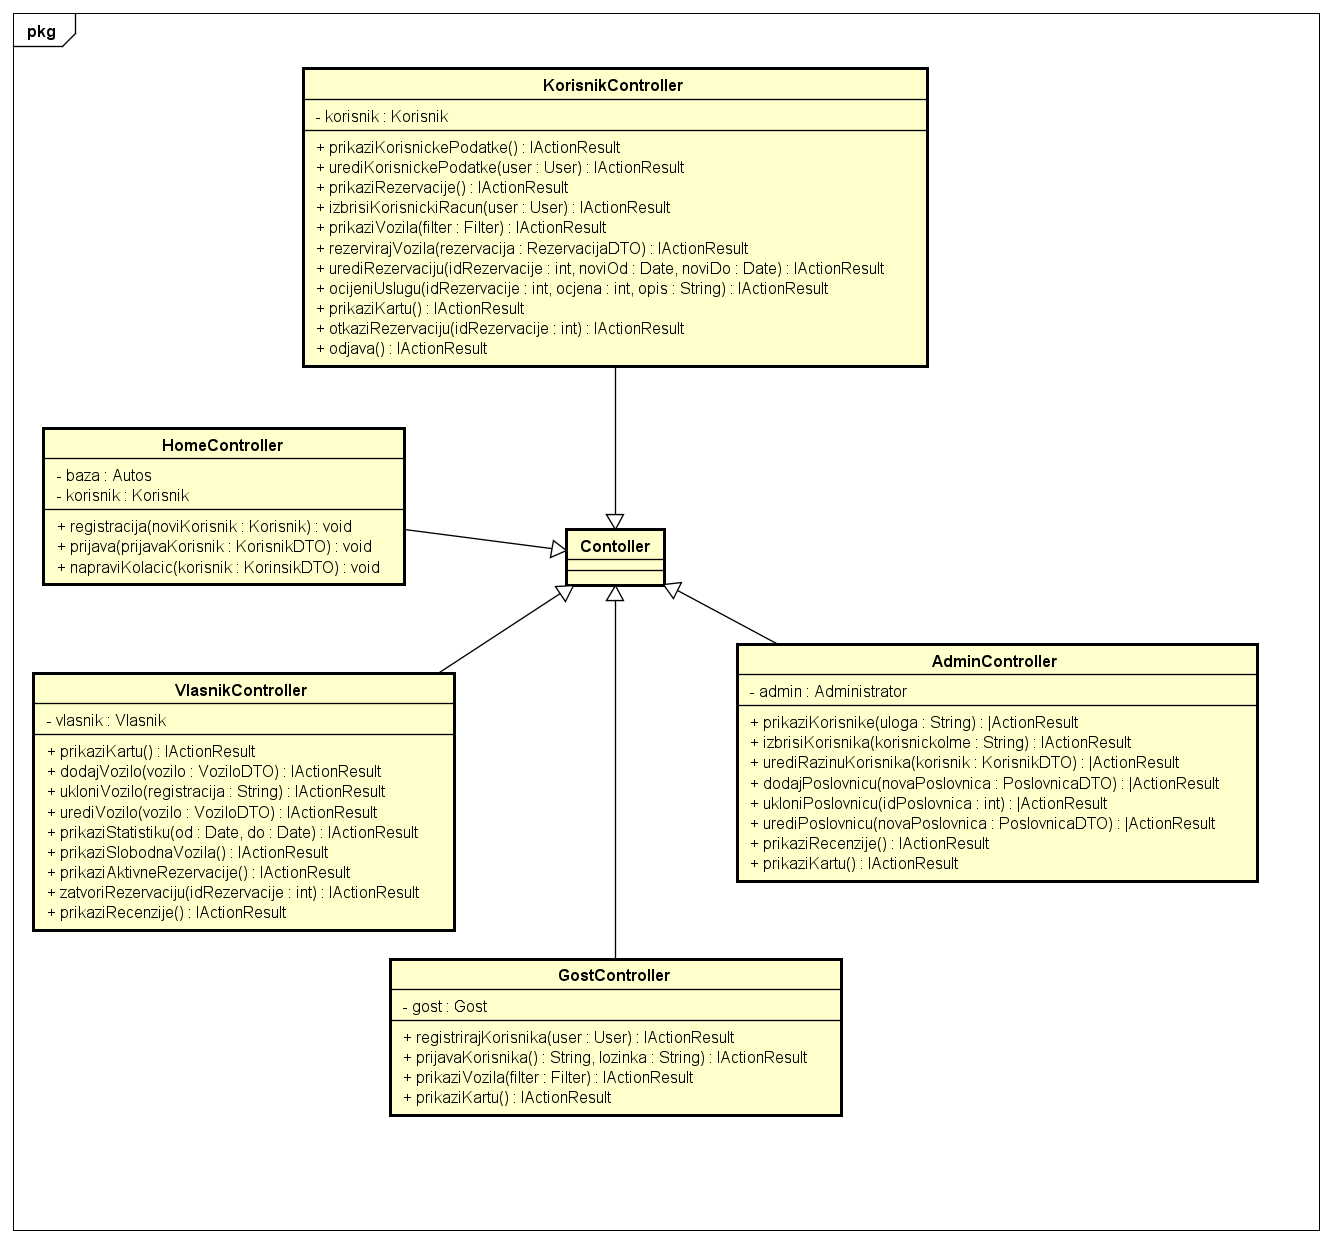
\includegraphics[width=16cm]{slike/dijagramRazreda1.png}
                \caption{Dijagram razreda - dio Contollers}
                \label{fig:classDiagram-1}
            \end{figure}
            \newpage
            
            \begin{figure}[hp]
                \centering
                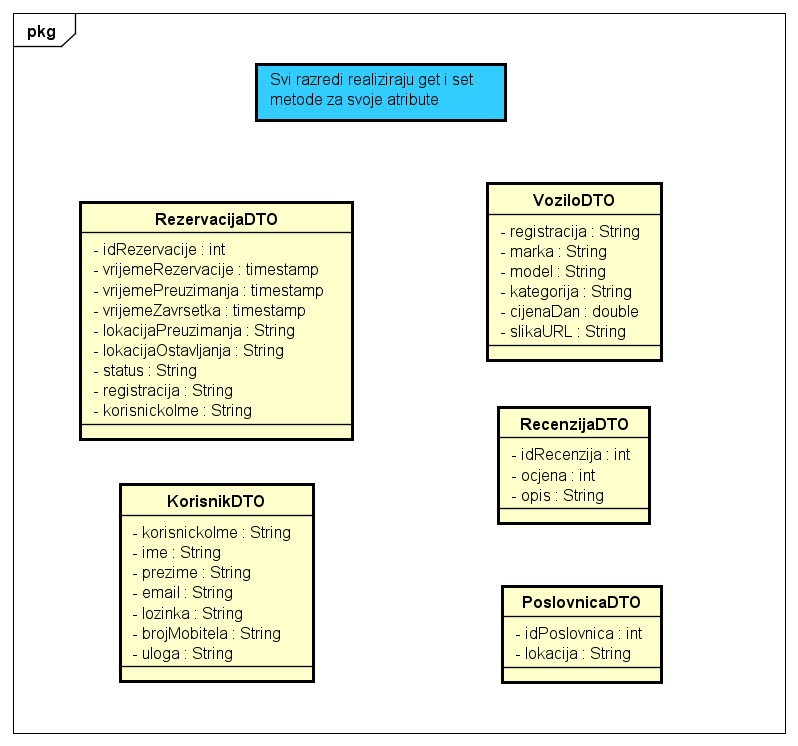
\includegraphics[width=16cm]{slike/dijagramRazreda2.png}
                \caption{Dijagram razreda - dio Data Transfer Objects}
                \label{fig:classDiagram-2}
            \end{figure}
            
            \noindent Dijagram razreda prikazuje strukturu baze podataka aplikacije.\\
            Razred OpćiKorisnik predstavlja registriranog korisnika. Svaki registrirani korisnik, neovisno o tomu bio on Korisnik, Vlasnik ili Administrator, nasljeđuje razred OpćiKorisnik. Razred Administrator predstavlja administratora sustava, koji ima najveće ovlasti. Razred Vlasnik predstavlja vlasnika sustava, koji ima ovlasti upravljanja vozilima i rezervacijama.
            Razred Korisnik predstavlja klijenta koji koristi osnovne funkcionalnosti aplikacije. \\
            Razred Gost predstavlja neregistriranog korisnika koji se može registrirati u sustav unoseći osnovne informacije.\\
            
            \newpage
            
            \begin{figure}[hp]
                \centering
                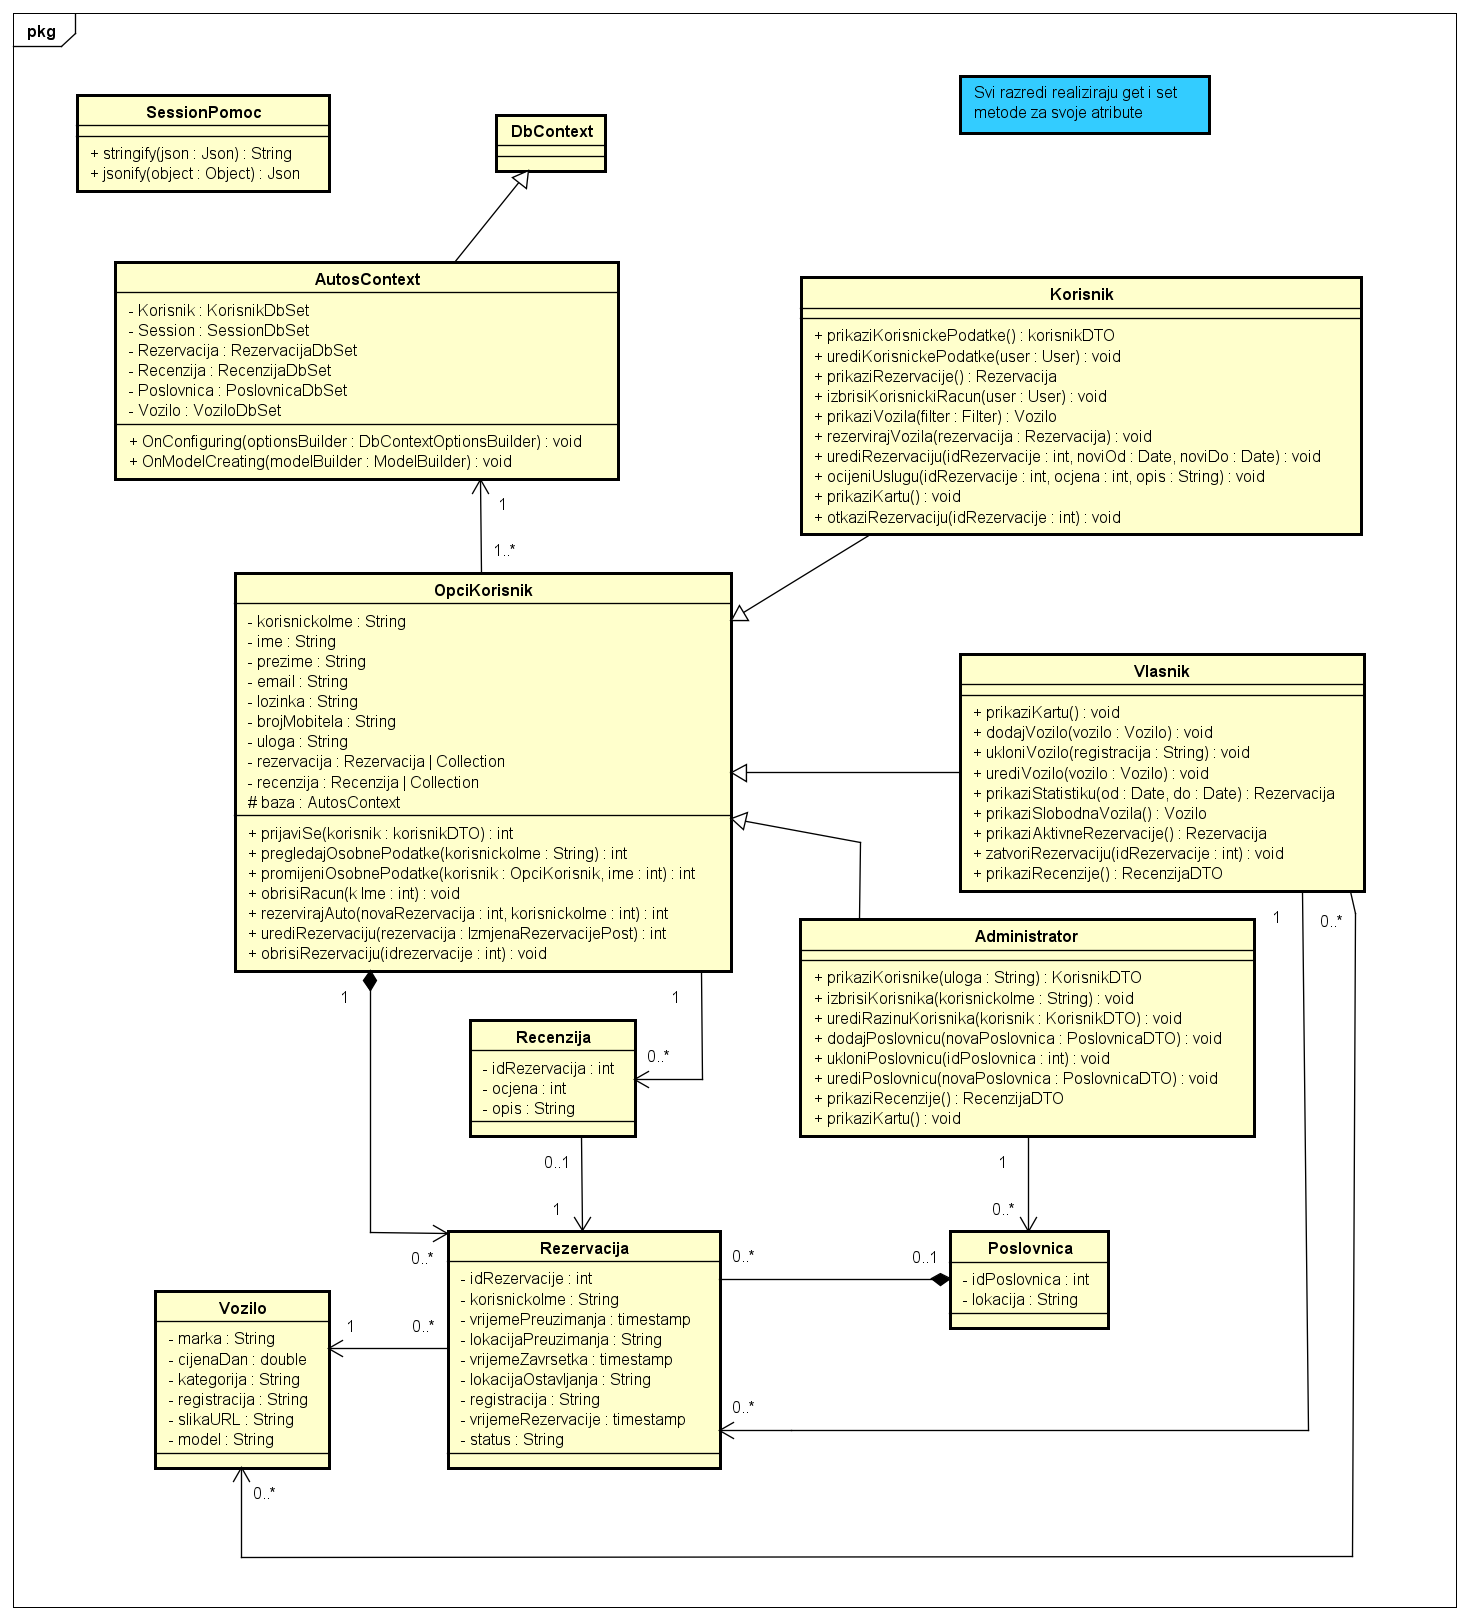
\includegraphics[width=15cm]{slike/dijagramRazreda3.png}
                \caption{Dijagram razreda - dio Models}
                \label{fig:classDiagram-3}
            \end{figure}
            \newpage
			
			\textbf{\textit{dio 2. revizije}}\\			
			
			\textit{Prilikom druge predaje projekta dijagram razreda i opisi moraju odgovarati stvarnom stanju implementacije}
			
			
			
			\eject
		
		\section{Dijagram stanja}
			
			
			\textbf{\textit{dio 2. revizije}}\\
			
			\textit{Potrebno je priložiti dijagram stanja i opisati ga. Dovoljan je jedan dijagram stanja koji prikazuje \textbf{značajan dio funkcionalnosti} sustava. Na primjer, stanja korisničkog sučelja i tijek korištenja neke ključne funkcionalnosti jesu značajan dio sustava, a registracija i prijava nisu. }
			
			
			\eject 
		
		\section{Dijagram aktivnosti}
			
			\textbf{\textit{dio 2. revizije}}\\
			
			 \textit{Potrebno je priložiti dijagram aktivnosti s pripadajućim opisom. Dijagram aktivnosti treba prikazivati značajan dio sustava.}
			
			\eject
		\section{Dijagram komponenti}
		
			\textbf{\textit{dio 2. revizije}}\\
		
			 \textit{Potrebno je priložiti dijagram komponenti s pripadajućim opisom. Dijagram komponenti treba prikazivati strukturu cijele aplikacije.}